
%\documentclass[manuscript]{acmart}
%\documentclass[acmsmall]{acmart}
%\settopmatter{printacmref=false}


\documentclass[
  a4paper,
  12pt,
  DIV=12,        % höherer Wert = schmalere Ränder, weniger Whitespacmi
  parskip=half,  % Absätze mit halbem Abstand statt Einzug
  headings=small % kleinere Überschriften, weniger vertikaler Abstand
]{scrartcl}

%\documentclass[a4paper,11pt]{scrartcl}
%\documentclass[a4paper,11pt]{report}
%\documentclass[a4paper,12pt]{book}
\usepackage[utf8]{inputenc}
\usepackage[german]{babel}
\usepackage[T1]{fontenc}
\usepackage{lmodern}
\usepackage[inkscapelatex=false]{svg}
% Texte im SVG von Inkscape setzen lassen, nicht durch die Dokumentschrift ersetzen
\svgsetup{inkscapelatex=false}
\usepackage{amsmath}
\usepackage{caption}
\usepackage{gensymb}
\usepackage{microtype}
\usepackage{longtable}
\usepackage{tabularx}   % Spalten, die die restliche Zeilenbreite auffüllen (X-Spalte)
\usepackage{booktabs}   % \toprule \midrule \bottomrule (in mobrob_table.tex verwendet)
\usepackage{wrapfig}    % Textumfluss um Abbildungen
\usepackage{array}
\usepackage{calc}


\usepackage[citecolor=black, colorlinks=true, linkcolor=black, urlcolor=blue]{hyperref}


%\usepackage{geometry}
\usepackage{siunitx}
%\geometry{margin=2.5cm}


\usepackage{amsthm}
\usepackage{mdframed}
\usepackage{enumitem}

\newmdtheoremenv{theorem}{Theorem}

\theoremstyle{definition}
\newmdtheoremenv{derivation}{Derivation}

\providecommand{\tightlist}{%
  \setlength{\itemsep}{0pt}\setlength{\parskip}{0pt}}

%\mdfdefinestyle{leftline}{
%    topline=false, bottomline=false, rightline=false,
%    linewidth=2pt, linecolor=gray
%}
\theoremstyle{definition}
\newmdtheoremenv[style=leftline]{myalgorithm}{Algorithm}




%\usepackage{fancyvrb}







\let\Bbbk\relax
\usepackage{amssymb}


\usepackage{yfonts}

\usepackage{kvmap}

\usepackage[
    backend=biber,
    style=alphabetic,
    sortlocale=de_DE,
    natbib=true,
    %url=false,
    doi=true,
    %eprint=false
]{biblatex}
% \addbibresource{Literaturrecherche-Stefan-Etringer/algo-references.bib}

%\usepackage[
%    backend=biber,
%    style=alphabetic,
%    sortlocale=de_DE,
%    natbib=true,
%    %url=false,
%    doi=true,
%    %eprint=false
%]{biblatex}
%\addbibresource{Literaturrecherche-Dennis/mobrob_references.bib}

\usepackage[autostyle=true,german=quotes]{csquotes}
\usepackage{trfsigns} %fourier transform arrow
\usepackage{mathrsfs} %fourier F
\usepackage{commath}

\usepackage{pgfplots}
\pgfplotsset{compat=1.18}

\usepackage{xcolor}
\usepackage{listings}
\usepackage[european]{circuitikz}
\ctikzset{tripoles/european not symbol=ieee circle}

%\usepackage[shading]{moeptikz}
%\moeptikzset{shading=true}

%\usepackage{german,longtable}

\usepackage{xcolor}
\usepackage{color}
\usepackage{url}

\usepackage{xfrac}

\usepackage{listings}
\usepackage{verbatimbox}

\usepackage{algorithm}
\usepackage{algpseudocode}

\usepackage{multirow}
\usepackage{float}
\usepackage{pdflscape}   % einzelne Querformatseiten (im PDF gedreht)

%%%% TIKZ

\usepackage{tikz}

\usepackage{pgfplots}
\usetikzlibrary{calc,
trees,positioning,arrows,
chains,shapes.geometric,
decorations.pathreplacing,
decorations.pathmorphing,shapes,
matrix,shapes.symbols,
plotmarks}
%\tikzexternalize[prefix=figures/]

%\tikzset{%
%  block/.style    = {draw, thick, rectangle, minimum height = 3em,
%    minimum width = 3em},
%  sum/.style      = {draw, circle, node distance = 2cm}, % Adder
%  input/.style    = {coordinate}, % Input
%  output/.style   = {coordinate} % Output
%}
% Defining string as labels of certain blocks.
%\newcommand{\suma}{\Large$+$}
%\newcommand{\multa}{\Large$\times$}
%\newcommand{\inte}{$\displaystyle \int$}
%\newcommand{\derv}{\huge$\frac{d}{dt}$}

\usetikzlibrary{arrows,automata,positioning}
%\usepackage{automata}


%%% END TIKZ

\usepackage[section]{placeins}

\usepackage{textcomp}


\usepackage{listings}
\usepackage{verbatimbox}

\usepackage{bold-extra}

\usepackage{framed}

\usepackage[table]{xcolor}

%\usepackage{fancyhdr}
%\pagestyle{fancy}
%\lhead{\leftmark}
%\chead{}
%\rhead{}
%\lfoot{}
%\cfoot{\thepage}
%\rfoot{}
%\renewcommand{\headrulewidth}{0.2pt}
%\renewcommand{\footrulewidth}{0.2pt}



\newcommand{\Z}{\mathbb{Z}}
\newcommand{\R}{\mathbb{R}}
\newcommand{\C}{\mathbb{C}}
\newcommand{\N}{\mathbb{N}}
\newcommand{\SqrtNy}{$\sqrt{\textsc{Ny}}$}
\newcommand{\conj}{\overline}
\newcommand{\Kset}{\textswab{K}}
\newcommand{\Qset}{\textswab{Q}}
\newcommand{\ceil}[1]{\left\lceil #1 \right\rceil}
\newcommand{\floor}[1]{\left\lfloor #1 \right\rfloor}
\newcommand{\sorted}[1]{\textsc{sort}\left\lbrace #1 \right\rbrace}
\newcommand{\SNRgain}{a_{SNR}}
\newcommand{\EQgain}{a_{EQ}}
\newcommand{\SIRgain}{a_{SIR}}
\newcommand{\SNIRgain}{a_{SINR}}
\newcommand{\SNR}{\textsc{SNR}}
\newcommand{\CIRgain}{a_{CIR}}
\newcommand{\CINRgain}{a_{CINR}}
\newcommand{\CNR}{\textsc{CNR}}
\newcommand{\CINR}{\textsc{CINR}}
\newcommand{\HPAModel}{ Hughes 1177H TWTA }
\newcommand{\bigO}{\mathcal{O}}
\newcommand{\CopWinCompl}{2.375377}
\newcommand{\IBO}{\textsc{IBO}}
\newcommand{\OBO}{\textsc{OBO}}
\newcommand{\spacepage}{\newpage\null\thispagestyle{empty}\newpage}
\newcommand{\satcom}{ SatCom }
\newcommand{\db}{~\text{dB}}


\definecolor{mGreen}{rgb}{0,0.6,0}
\definecolor{mGray}{rgb}{0.5,0.5,0.5}
\definecolor{mPurple}{rgb}{0.58,0,0.82}
\definecolor{backgroundColour}{rgb}{0.95,0.95,0.92}

\lstdefinestyle{CStyle}{
    backgroundcolor=\color{backgroundColour},
    commentstyle=\color{mGreen},
    keywordstyle=\color{magenta},
    numberstyle=\tiny\color{mGray},
    stringstyle=\color{mPurple},
    basicstyle=\footnotesize,
    breakatwhitespace=false,
    breaklines=true,
    captionpos=b,
    keepspaces=true,
    numbers=left,
    numbersep=5pt,
    showspaces=false,
    showstringspaces=false,
    showtabs=false,
    tabsize=2,
    language=C
}

\lstdefinelanguage{VHDL}{
  morekeywords=[1]{library,use,all,entity,is,port,in,out,end,architecture,of,begin,process,if,then,else,elsif,when,others,signal,variable,wait,for,loop},
  morecomment=[l]--,
  morestring=[b]",
  sensitive=true
}

\lstset{
  language=VHDL,
  basicstyle=\ttfamily\small,
  keywordstyle=\color{blue},
  commentstyle=\color{gray},
  stringstyle=\color{red},
  numbers=left,
  numberstyle=\tiny,
  stepnumber=1,
  numbersep=8pt,
  frame=single,
  breaklines=true,
  captionpos=b
}

\lstset{numbers=none}

%\newcounter{example}
%\renewcommand{\theexample}{\thesection.\arabic{example}}


% Default fixed font does not support bold face
\DeclareFixedFont{\ttb}{T1}{txtt}{bx}{n}{12} % for bold
\DeclareFixedFont{\ttm}{T1}{txtt}{m}{n}{12}  % for normal

% Custom colors
\usepackage{color}
\definecolor{deepblue}{rgb}{0,0,0.5}
\definecolor{deepred}{rgb}{0.6,0,0}
\definecolor{deepgreen}{rgb}{0,0.5,0}

\usepackage{listings}

% Python style for highlighting
\newcommand\pythonstyle{\lstset{
language=Python,
basicstyle=\ttm,
morekeywords={self},              % Add keywords here
keywordstyle=\ttb\color{deepblue},
emph={MyClass,__init__},          % Custom highlighting
emphstyle=\ttb\color{deepred},    % Custom highlighting style
stringstyle=\color{deepgreen},
frame=tb,                         % Any extra options here
showstringspaces=false
}}


% Python environment
\lstnewenvironment{python}[1][]
{
\pythonstyle
\lstset{#1}
}
{}

% Python for external files
\newcommand\pythonexternal[2][]{{
\pythonstyle
\lstinputlisting[#1]{#2}}}

% Python for inline
\newcommand\pythoninline[1]{{\pythonstyle\lstinline!#1!}}


% ---------------------------------------------------------------------
% Stil fuer C++-Listings dieser Dokumentation
% ---------------------------------------------------------------------
\lstdefinestyle{cpp}{
  language=C++,
  basicstyle=\ttfamily\footnotesize,
  keywordstyle=\color{deepblue},
  commentstyle=\color{mGreen},
  stringstyle=\color{mPurple},
  numbers=none,
  breaklines=true,
  showstringspaces=false,
  frame=single,
  columns=fullflexible,
  captionpos=b
}



%\nocite{*}


\begin{document}
%\pagenumbering{roman}



\title{Coasterbot}
\subtitle{Maturityreport}
\author{Dennis Borutta}
%\email{gereonsuch@suchdsp.com}
%\affiliation{
%  \institution{Wilhelm Büchner University of Applied Sciences}
%  \department{Computer Engineering}
%  \city{Hof}
%  \country{Germany}
%}



\begin{titlepage}
  \begin{center}
    {\large Wilhelm Büchner University of Applied Sciences} \\[0.3em]

    {\normalsize Projektseminar Master}
\vspace{5em}

    {\LARGE\bfseries Coasterbot} \\[0.5em]

    {\large Maturityreport} \\[1em]

    {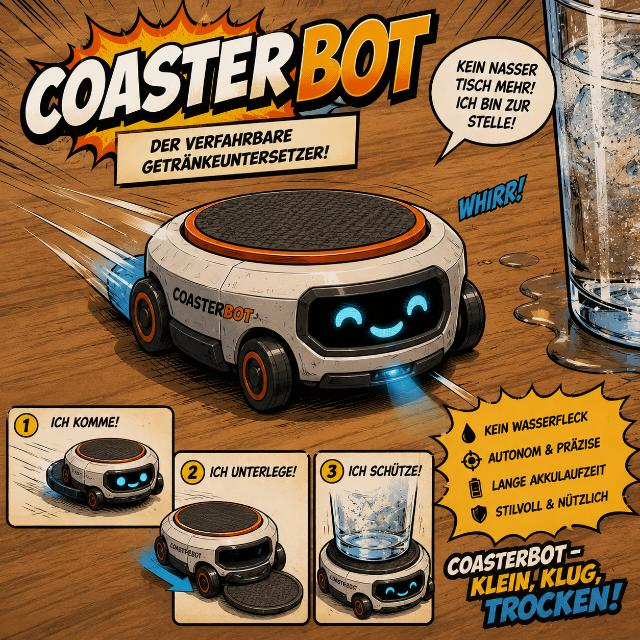
\includegraphics[width=0.38\textwidth]{coasterbot.png}} \\[1em]

\vspace{4em}

    {\normalsize
\begin{tabular}{ll}
Dennis Borutta, B. Eng & dennis.borutta@outlook.com\\
Stefan Etringer, B. Eng & mail@stefan.works\\
Gereon Such, M. Sc. & gereonsuch@gmail.com\\
\end{tabular}
    }
  \end{center}


\end{titlepage}


% einleitung preambel etc.


% Versionshistorie des Dokuments: eigene Seite direkt nach dem Titelblatt
\section*{Versionshistorie}
\begin{tabularx}{\textwidth}{@{}clp{2.6cm}X@{}}
\toprule
\textbf{Version} & \textbf{Datum} & \textbf{Bearbeiter} & \textbf{Änderungen}\\
\midrule
1 & 25.09.2026 & Borutta & Erstfassung: Maturityreport auf Basis des Lastenhefts (Kapitel 2.7).\\
\bottomrule
\end{tabularx}

\newpage

\tableofcontents

\newpage

% Etwas mehr Toleranz beim Umbruch: viele \texttt{}-Bezeichner sind nicht
% trennbar und wuerden sonst knapp ueber den Satzspiegel ragen.
\setlength{\emergencystretch}{3em}

% =====================================================================
\section{Einleitung}\label{einleitung}
% =====================================================================

\subsection{Zweck des Dokuments}\label{zweck-des-dokuments}

Dieser Maturityreport dokumentiert das erreichte Maturity-Level der im
Lastenheft definierten Ausbaustufen. Während das Lastenheft festlegt,
welchen Funktionsumfang definierte Ausbaustufen haben, hält dieser Report fest, welchen Funktionsumfang der Prototyp abdeckt. 
Dies wird erreicht durch den Aufbau einer Matrix, in der die erste Spalte die verschiedenen Funktionen definiert und 
die darauffolgenden Spalten die verschieden Maturity-Level darstellen. In den Zellen werden die erreichten Funktionen abgehakt und bei Bedarf mit Anmerkungen versehen.
Alle Zellen die eine nicht notwendige Funktion für ein Maturity-Level darstellen, sind ausgegraut. Eine teilweise oder komplette Umsetzung der Funktion ist möglich, aber nicht
erforderlich zum Erreichen des Maturity-Levels.

Es ist dabei zu beachten, dass das Ziel dieses Projektes das Erreichen der ersten Ausbaustufe ist. 
Daher ist zu erwarten, dass ein Großteil des Funktionsumfang noch nicht erreicht wurde. Dennoch hilft dieser Report dabei,
den Entwicklungsstand des Coasterbots zu verfolgen.

\subsection{Definition der Maturity-Level}\label{definition-der-maturity-level}
Im Lastenheft sind folgende Maturity-Level definiert:

\textbf{Maturity Level 1 -- Prototyp}

Nachweis der autonomen Navigation, Lokalisierung, sicheren Bewegung
sowie der Aufnahme und Ausgabe von Getränkeuntersetzern.

\textbf{Maturity Level 2 -- Erweiterter Funktionsumfang}

Erweiterung um Funktionen zur Energieverwaltung sowie zur
automatisierten Tischreinigung.

\textbf{Maturity Level 3 -- Servicefunktionen}

Integration von Funktionen zur digitalen Bestellaufnahme und
Unterstützung von Bezahlvorgängen.

\textbf{Maturity Level 4 -- Mensch-Roboter-Interaktion}

Erweiterung der Interaktion zwischen Gästen und Roboter, beispielsweise
durch personenbezogene Zuordnung von Anfragen oder individuelle
Statuskommunikation.

\textbf{Maturity Level 5 -- Getränketransport}

Erweiterung des Systems um den sicheren autonomen Transport kompletter
Getränke unter Berücksichtigung der fahrdynamischen Anforderungen.



\section{Maturityreport}\label{maturityreport}
% Farben definieren (optional)
\definecolor{greybg}{HTML}{EFEFEF}

% **************************************
\sloppy % Behebt Overfull HBox Warnungen durch Flexibilität bei Abständen
\begin{longtable}{@{}p{6cm}|p{1cm}p{1cm}p{1cm}p{1cm}p{1cm}@{}|ccccc@{}} 
\caption{Maturity Level Übersicht} \\
\toprule 
& \multicolumn{5}{c}{\centering Maturity Level} \\ 
\midrule[1pt] % Dicke Linie unter dem Header

Funktion & M1 & M2 & M3 & M4 & M5 \\
\toprule 
\endfirsthead

% --- KEINE CONTINUED FROM PREVIOUS PAGE ZEILE mehr, um die Warnungen zu vermeiden ---
\endhead


% --- Der eigentliche Inhalt der Tabelle (Daten) ---

Autonome Navigation & \centering\textbf{X} & &  &  &  \\
\toprule

Lokalisierung der Untersetzer & \centering\textbf{(X)} &  &  &  &  \\ 
\toprule

Aufnahme von Untersetze & \centering\textbf{X} &  &  &  &  \\
\toprule

Ausgabe von Untersetzer & \centering\textbf{X} &  &  &  &  \\
\toprule

Energieverwaltung & \cellcolor{greybg} \centering\textbf{(X)} &  &  &  &  \\
\toprule

Tischreinigung & \cellcolor{greybg} &  &  &  &  \\
\toprule

Digitale Bestellaufnahme & \cellcolor[HTML]{EFEFEF} & \cellcolor[HTML]{EFEFEF} &  &  &  \\
\toprule

Unterstützung bei Bezahlvorgängen & \cellcolor[HTML]{EFEFEF} & \cellcolor[HTML]{EFEFEF} &  &  &  \\
\toprule

Statusabfragen durch Benutzer & \cellcolor[HTML]{EFEFEF} & \cellcolor[HTML]{EFEFEF} & \cellcolor[HTML]{EFEFEF} &  &  \\
\toprule

Benutzerzentrierte Entertainmentfunktionen & \cellcolor[HTML]{EFEFEF} & \cellcolor[HTML]{EFEFEF} & \cellcolor[HTML]{EFEFEF} &  &  \\
\toprule

Transport von Getränken & \cellcolor[HTML]{EFEFEF} & \cellcolor[HTML]{EFEFEF} & \cellcolor[HTML]{EFEFEF} & \cellcolor[HTML]{EFEFEF} &  \\
\toprule

Verschüttungssicherung beim Transport von Getränken & \cellcolor[HTML]{EFEFEF} & \cellcolor[HTML]{EFEFEF} & \cellcolor[HTML]{EFEFEF} & \cellcolor[HTML]{EFEFEF} &  \\
\bottomrule % Abschlusslinie

\end{longtable}

\newpage

\subsection{Anmerkungen zu Maturity Level 1}\label{anmerkungen}
\begin{itemize}
\item \textbf{Autonome Navigation:} Die autonome Navigation wurde erfolgreich implementiert und getestet. Der Coasterbot kann sich selbstständig in der Umgebung bewegen und Hindernissen ausweichen.
\item \textbf{Lokalisierung der Untersetzer:} Die Lokalisierung der Untersetzer erfolgt durch festgelegte Koordinaten. Hier besteht Verbesserungsbedarf.
\item \textbf{Aufnahme von Untersetzern:} Die Mechanismen zur Aufnahme von Untersetzern funktionieren.
\item \textbf{Ausgabe von Untersetzern:} Die Mechanismen zur Ausgabe von Untersetzern funktionieren.
\item \textbf{Energieverwaltung:} Die Energie wird über eine wiederaufladbare Batterie bereitgestellt. Eine automatische Energieverwaltung ist noch nicht implementiert. Jedoch kann über ein Entlademodell und der eingebauten LED, eine grobe Ladezustandsüberwachung implementiert werden.
\end{itemize}

\newpage
\section{Fazit}\label{fazit}
Der Coasterbot erfüllt die Mindestanforderungen für das verfolgte Maturity-Level 1 teilweise. 
Die Kernfunktionen sind abgedeckt, jedoch besteht ein Verbesserungsbedarf bei der Lokalisierung der Untersetzer.
Diese sollten in zukünftigen Versionen durch andere Mechanismen lokalisiert werden. Vorstellbar wäre der Einsatz
einer Kamera, die die Untersetzer erkennt und deren Position schätzt. Hinzu sollten Sensoren kommen, die sicherstellen,
dass der Coasterbot sich über den Untersetzer befindet, bevor er diesen aufnimmt.

\end{document}
